\newpage

\section{Appendix}

\subsection{Seconds per epoch}

Continuing section \ref{ss:comp_req}, we report the exact values per epoch across experiment configurations. We do so, since different architectures and datasets may require training for different number of epochs, however the epoch time remains the same across experiments.

\begin{table*}[hbt!]
\begin{center}
\begin{tabular}{|c|c|c|c|c|c|c|}
\hline
\textbf{Experiment}      & \textbf{Setup (way,shot)} & \textbf{Seconds per epoch (Conv4 / ProtoNet)}   \\
\hline\hline

ProtoNet                 & (5,5)          &          20/25                                 \\\hline

ProtoNet                 & (20,5)         &           45/50                               \\\hline
ProtoNet+Jigsaw          & (5,5)          &            25/35                             \\\hline
ProtoNet+Jigsaw          & (20,5)         &             60/66                               \\\hline
ProtoNet+Rotation        & (5,5)          &              18/60                             \\\hline
ProtoNet+Rotation        & (20,5)         &             65/81                            \\\hline
ProtoNet+Jigsaw+Rotation & (5,5)          &              42/70                            \\\hline
ProtoNet+Jigsaw+Rotation & (20,5)         &              83/95  \\
\hline
\end{tabular}
\end{center}
\caption{Average seconds per epoch across experimental setups and ways}
\label{table:epoch_time}
\end{table*}

\subsection{Hyperparameter sweeps}

The selected experiment configs are as follows:

Each of the below experimental configurations are done for ProtoNet, ProtoNet+Jigsaw, ProtoNet+Rotation and ProtoNet+Jigsaw+Rotation (4 configurations) in the \underline{5-way 5-shot} setup. The sweeps optimize the \textbf{learning rate} and \textbf{the mode of batch normalization}, and \textbf{Alpha}, $\alpha$. 

The last two parameters are optimized only when self-supervision is applied. This is because $\alpha=0$ for fully supervised learners and we find that using batch norm modes 2,3 is highly detrimental to fully supervised learners.

\begin{itemize}
\item miniImageNet Conv4: \textbf{4} sweeps
\item miniImageNet ResNet-18: \textbf{4} sweeps  
% \item miniImageNet ResNet-18 - ProtoNet, ProtoNet+Jigsaw, ProtoNet+Rotation, ProtoNet+Jigsaw+Rotation - for 20-way: \textbf{4} sweeps
\item CUB Conv4: \textbf{4} sweeps
\item Cars Conv4: \textbf{4} sweeps
\item CUB ResNet-18: \textbf{4} sweeps
\item Cars ResNet-18: \textbf{4} sweeps
\end{itemize}

Hence we do a total of \textbf{24} sweeps.

The sweeps and the exact hyperparameters obtained can be visualized at \url{https://wandb.ai/meta-learners/FSL-SSL/sweeps}. All the runs in the paper can be seen at \url{https://wandb.ai/meta-learners}. Our code can be accessed at \url{https://github.com/ashok-arjun/MLRC-2021-Few-Shot-Learning-And-Self-Supervision}.

% \clearpage

\subsection{Tables}

\subsubsection{Results on the applying self-supervision - with the Conv4 architecture}

\begin{table*}[hbt!]
\begin{center}
\begin{tabular}{|c|c|c|c|c|c|}
\hline
Method & CUB & Cars & Aircrafts & Dogs & Flowers \\
\hline\hline
ProtoNet & \textbf{77.72 \textpm\ 0.48} & \textbf{67.99 \textpm\ 0.41} & \textbf{76.16 \textpm\ 0.69} & \textbf{63.88 \textpm\ 0.54} & \textbf{85.29 \textpm\ 0.51} \\
ProtoNet + Jigsaw & 75.57 \textpm\ 0.7 & 62.54 \textpm\ 0.39 & 74.53 \textpm\ 0.68 & 54.27 \textpm\ 0.51 & 84.4 \textpm\ 0.47 \\
ProtoNet + Rotation & 77.5 \textpm\ 0.55 & 66.8 \textpm\ 0.40 & 74.16 \textpm\ 0.40 & 60.74 \textpm\ 0.58 & 84.55 \textpm\ 0.5 \\
ProtoNet + Jigsaw + Rotation & 69.66 \textpm\ 0.45 & 59.76 \textpm\ 0.77 & 74.79 \textpm\ 0.4 & 49.48 \textpm\ 0.54 & 81.43 \textpm\ 0.51 \\
\hline
\end{tabular}
\end{center}
\caption{Conv-4's performance on few-shot learning tasks. 
Applying self-supervision to few-shot learners results in decrease in performance} 
\label{table:conv_few_shot}
\end{table*}



\begin{table*}[hbt!]
\begin{center}
\begin{tabular}{|c|c|c|c|}
\hline
Method & CUB & Cars \\
\hline\hline
%  & \multicolumn{3}{c|}{5-way 5-shot} \\\hline
ProtoNet & \textbf{76.43 \textpm\ 0.3} & \textbf{67.45 \textpm\ 0.85} \\
ProtoNet + Jigsaw & 65.09 \textpm\ 0.42 & 60.39 \textpm\ 0.76 \\
ProtoNet + Rotation & 75.05 \textpm\ 0.35 & 66.61 \textpm\ 0.6  \\
\hline
\end{tabular}
\end{center}
\caption{Conv4 results on CUB and cars with a different seed}
\label{table:seed_conv}
\end{table*}


\begin{table*}[hbt!]
\begin{center}
\begin{tabular}{|c|c|c|}
\hline
Method & Conv-4 \\
\hline\hline
ProtoNet &  \textbf{66.78 \textpm\ 0.84} \\
ProtoNet + Jigsaw & 64.94 \textpm\ 0.75 \\
ProtoNet + Rotation & 66.41 \textpm\ 0.73 \\
ProtoNet + Jigsaw + Rotation & 65.21 \textpm\ 0.73 \\

\hline
\end{tabular}
\end{center}
\caption{miniImageNet Results on Conv4}
\label{table:mini_imagenet_both}
\end{table*}


\subsubsection{Results on harder tasks}

\begin{table*}[hbt!]
\begin{center}
\begin{tabular}{|c|c|c|c|}
\hline
Method & 20\% CUB & 20\% Cars & 20\% Dogs \\
\hline\hline
No SSL & \textbf{73.61 \textpm\ 0.71} & 75.16 \textpm\ 0.84 & 68.4 \textpm\ 0.64 \\
20\% SSL & 70.84 \textpm\ 0.73 & 83.72 \textpm\ 0.75 & 68.13 \textpm\ 0.9 \\
40\% SSL & 71.48 \textpm\ 0.9 & 83.87 \textpm\ 0.73 & 68.26 \textpm\ 0.87 \\
60\% SSL & 70.71 \textpm\ 0.81 & \textbf{84.12 \textpm\ 0.73} & \textbf{74.21 \textpm\ 0.89} \\
80\% SSL & 71.99 \textpm\ 0.65 & 84.04 \textpm\ 0.78 & 71.86 \textpm\ 0.81 \\
\hline
\end{tabular}
\end{center}
\caption{Performance on tasks with lesser labelled data. SSL increases performance under this setup on $2$ out of $3$ datasets}
\label{table:20_ssl}
\end{table*}


\begin{table*}[hbt!]
\begin{center}
\begin{tabular}{|c|c|c|c|}
\hline
Method & 20\% CUB & 20\% Cars & 20\% Dogs \\
\hline\hline
No SSL & \textbf{73.61 \textpm\ 0.82} & 75.16 \textpm\ 0.84 & 68.4 \textpm\ 0.64 \\
20\% SSL & 69.83 \textpm\ 0.79 & \textbf{81.53 \textpm\ 0.79} & 71.99 \textpm\ 0.88 \\
40\% SSL & 71.08 \textpm\ 0.83 & 75.27 \textpm\ 0.89 & 72.24 \textpm\ 0.85 \\
60\% SSL & 71.12 \textpm\ 0.91 & 76.39 \textpm\ 0.89 & \textbf{73.11 \textpm\ 0.83} \\
80\% SSL & 68.48 \textpm\ 0.87 & 73.85 \textpm\ 0.89 & 72.03 \textpm\ 0.91 \\
\hline
\end{tabular}
\end{center}
\caption{Performance when a portion of data replaced with data from other domains. SSL increases performance under this setup on $2$ out of $3$ datasets}
\label{table:20_ssl_others}
\end{table*}


\begin{table*}[hbt!]
\begin{center}
\begin{tabular}{|c|c|c|c|}
\hline
Method & CUB Greyscale & Cars Low-resolution & Dogs Greyscale \\
\hline\hline
%  & \multicolumn{3}{c|}{5-way 5-shot} \\\hline
ProtoNet & 82.88 \textpm\ 0.56 & 86.00 \textpm\ 0.51 & 79.97 \textpm\ 0.54 \\
ProtoNet + Jigsaw & \textbf{85.44 \textpm\ 0.52} & \textbf{86.34 \textpm\ 0.56} & \textbf{82.82 \textpm\ 0.50} \\
ProtoNet + Rotation & 83.51 \textpm\ 0.55 & 85.53 \textpm\ 0.53 & 81.74 \textpm\ 0.59 \\
\hline
\end{tabular}
\end{center}
\caption{Performance on artificially constructed harder tasks. Applying SSL increases performance in this setup}
\label{table:grey_low_res}
\end{table*}


\subsubsection{Results on domain selection}

\begin{table}[H]
\begin{center}
\begin{tabular}{|c|c|c|c|c|c|}
\hline
Method & CUB & Cars & Aircrafts & Dogs & Flowers \\
\hline\hline
No SSL & 69.05 \textpm\ 0.48 & 75.15 \textpm\ 0.41 & 74.8 \textpm\ 0.35 & 68.4 \textpm\ 0.54 & 76.34 \textpm\ 0.51 \\
SSL Pool (Random) & 71.11 \textpm\ 0.43 & 75.27 \textpm\ 0.39 & 75.81 \textpm\ 0.39 & 68.38 \textpm\ 0.51 & 79.71 \textpm\ 0.47 \\
SSL Pool (Weight) & \textbf{71.25 \textpm\ 0.55} & \textbf{75.65 \textpm\ 0.40} & \textbf{80.13 \textpm\ 0.40} & \textbf{70.66 \textpm\ 0.58} & \textbf{82.16 \textpm\ 0.5} \\

\hline
\end{tabular}
\end{center}
\caption{Domain selection results. The implementation of the domain selection algorithm is verified, and using the algorithm to select unlabelled data for SSL gives the best results across all datasets}
\label{table:domain}
\end{table}

\subsubsection{Results on cross-domain few-shot learning}

\begin{table*}[hbt!]
\begin{center}
\begin{tabular}{|c|c|c|c|c|}
\hline
Method & ChestX & Crop Disease & EuroSAT & ISIC \\
\hline\hline
ProtoNet & \textbf{24.46 \textpm\ 0.39} & \textbf{80.45 \textpm\ 0.66} & 67.03 \textpm\ 0.7 & \textbf{41.0 \textpm\ 0.6} \\
ProtoNet + Jigsaw & 24.07 \textpm\ 0.4 & 78.51 \textpm\ 0.66 & 64.69 \textpm\ 0.7 & 39.81 \textpm\ 0.54 \\
ProtoNet + Rotation & \textbf{24.46 \textpm\ 0.39} & 79.30 \textpm\ 0.7 & 66.50 \textpm\ 0.71 & 39.54 \textpm\ 0.54 \\
ProtoNet + Jigsaw + Rotation & 24.16 \textpm\ 0.37 & 78.67 \textpm\ 0.66 & \textbf{67.60 \textpm\ 0.66} & 40.22 \textpm\ 0.54 \\

\hline
\end{tabular}
\end{center}
\caption{CDFSL Benchmark for Conv-4. Applying SSL decreases performance in the cross-domain few-shot inference setup, and fully-supervised learning is state-of-the-art in $3$ out of $4$ datasets}
\label{table:cdfsl_conv}
\end{table*}

% \clearpage

\subsection{Architectures}

\vspace*{1.0cm}

% \begin{table}[H]
% \parbox{.45\linewidth}{
%     \centering

% 	\begin{tabular}{|c|c|c|}
% 	\hline
% 	Layer Name             & Output Size                   & Conv-4-64                 \\ \hline\hline
% 	conv1                  & 82 x 82 x 64                  & 3 x 3, 64                 \\ \hline
% 	\multirow{2}{*}{conv2} & \multirow{2}{*}{41 x 41 x 64} & 2 x 2, max pool, stride 2 \\ \cline{3-3} 
% 		               &                               & 3 x 3, 64                 \\ \hline
% 	\multirow{2}{*}{conv3} & \multirow{2}{*}{18 x 18 x 64} & 2 x 2, max pool, stride 2 \\ \cline{3-3} 
% 		               &                               & 3 x 3, 64                 \\ \hline
% 	\multirow{2}{*}{conv4} & \multirow{2}{*}{7 x 7 x 64}   & 2 x 2, max pool, stride 2 \\ \cline{3-3} 
% 		               &                               & 3 x 3, 64                 \\ \hline
% 	average pool           & 1 x 1 x 64                    & 7 x 7 average pool        \\ \hline
% 	fully connected        & 1024                             & 64 x 1024 linear  \\ \hline
% 	fully connected        & X                             & 1024 x X linear  \\ \hline
% 	softmax                & X                             &                           \\ \hline
% 	\end{tabular}
% 	\caption{Conv-4 Architecture (X denotes the way)}
% 	\label{table:conv_arch}

% }
% \hfill
% \parbox{.45\linewidth}{
% \centering

% 	\begin{tabular}{|c|c|c|}
% 	\hline
% 	Layer Name             & Output Size                   & Conv-4-64                 \\ \hline\hline
% 	conv1                     & 112 x 112 x 64                & 7 x 7, 64, stride 2        \\ \hline
% 	\multirow{2}{*}{conv2\_x} & \multirow{2}{*}{56 x 56 x 64} & 3 x 3 max pool, stride 2   \\ \cline{3-3} 
% 		                  &                               & [3 x 3, 64$;$ 3 x 3, 64] x 2   \\ \hline
% 	conv3\_x                  & 28 x 28 x 128                 & [3 x 3, 128$;$ 3 x 3, 128] x 2 \\ \hline
% 	conv4\_x                  & 14 x 14 x 256                 & [3 x 3, 256$;$ 3 x 3, 256] x 2 \\ \hline
% 	conv5\_x                  & 7 x 7 x 512                   & [3 x 3, 512$;$ 3 x 3, 512] x 2 \\ \hline
% 	average pool              & 1 x 1 x 512                   & 7 x 7 average pool         \\ \hline
% 	fully connected           & X                             & 512 x X fully connections  \\ \hline
% 	softmax                   & X                             &                            \\ \hline
% 	\end{tabular}
% 	\caption{ResNet-18 Architecture}
% 	\label{table:resnet_arch}
% }
% \end{table} 



\begin{table*}[hbt!]
\begin{center}
\begin{tabular}{|c|c|c|}
\hline
Layer Name             & Output Size                   & Conv-4-64                 \\ \hline\hline
conv1                  & 82 x 82 x 64                  & 3 x 3, 64                 \\ \hline
\multirow{2}{*}{conv2} & \multirow{2}{*}{41 x 41 x 64} & 2 x 2, max pool, stride 2 \\ \cline{3-3} 
                       &                               & 3 x 3, 64                 \\ \hline
\multirow{2}{*}{conv3} & \multirow{2}{*}{18 x 18 x 64} & 2 x 2, max pool, stride 2 \\ \cline{3-3} 
                       &                               & 3 x 3, 64                 \\ \hline
\multirow{2}{*}{conv4} & \multirow{2}{*}{7 x 7 x 64}   & 2 x 2, max pool, stride 2 \\ \cline{3-3} 
                       &                               & 3 x 3, 64                 \\ \hline
average pool           & 1 x 1 x 64                    & 7 x 7 average pool        \\ \hline
fully connected        & 1024                             & 64 x 1024 linear  \\ \hline
fully connected        & X                             & 1024 x X linear  \\ \hline
softmax                & X                             &                           \\ \hline
\end{tabular}
\end{center}
\caption{Conv-4 Architecture (X denotes the way)}
\label{table:conv_arch}
\end{table*}

% \begin{figure*}[hbt!]
%     \centering
%     \begin{minipage}{0.9\textwidth}
%         \centering
%         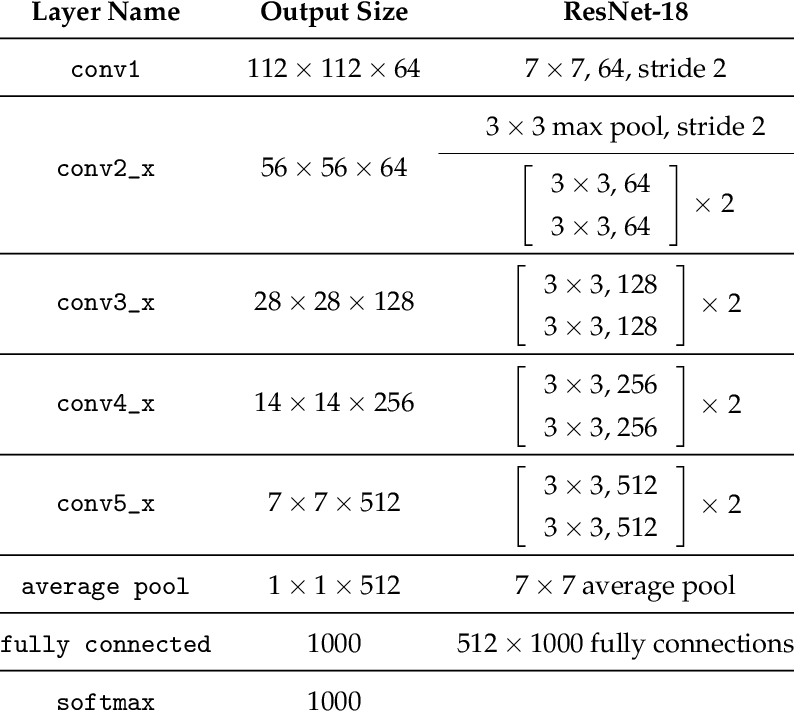
\includegraphics[width=0.6\textwidth, height=7.5cm]{pdfs/resnet18.png}
%         \caption{\centering ResNet-18 Architecture. \\ Instead of $1000$, the final layer \\ is set to $X$ classes where $X$ denotes the way}
%         \label{fig:resent18_arch}
%     \end{minipage}\hfill
% \end{figure*}

\vspace*{1.0cm}


\begin{table*}[hbt!]
\begin{center}
\begin{tabular}{|c|c|c|}
\hline
Layer Name             & Output Size                   & Conv-4-64                 \\ \hline\hline
conv1                     & 112 x 112 x 64                & 7 x 7, 64, stride 2        \\ \hline
\multirow{2}{*}{conv2\_x} & \multirow{2}{*}{56 x 56 x 64} & 3 x 3 max pool, stride 2   \\ \cline{3-3} 
                          &                               & [3 x 3, 64$;$ 3 x 3, 64] x 2   \\ \hline
conv3\_x                  & 28 x 28 x 128                 & [3 x 3, 128$;$ 3 x 3, 128] x 2 \\ \hline
conv4\_x                  & 14 x 14 x 256                 & [3 x 3, 256$;$ 3 x 3, 256] x 2 \\ \hline
conv5\_x                  & 7 x 7 x 512                   & [3 x 3, 512$;$ 3 x 3, 512] x 2 \\ \hline
average pool              & 1 x 1 x 512                   & 7 x 7 average pool         \\ \hline
fully connected           & X                             & 512 x X fully connections  \\ \hline
softmax                   & X                             &                            \\ \hline
\end{tabular}
\end{center}
\caption{ResNet-18 Architecture}
\label{table:resnet_arch}
\end{table*}